\documentclass{ol-softwaremanual}

% Page layout
\usepackage[a4paper, top=3.5cm, bottom=3.5cm, left=2.5cm, right=2.5cm]{geometry}

% Packages used in this example
\usepackage{graphicx}  % for including images
\usepackage{hyperref}  % for hyperlinks
\usepackage{amsmath}   % for equations and mathematics
\usepackage{microtype} % for typographical enhancements
\usepackage{xcolor}
\usepackage{minted}    % for code listings
\usemintedstyle{borland}

\definecolor{codegray}{rgb}{0.5,0.5,0.5}
\definecolor{LightGray}{gray}{0.9}


% Others
\setminted{style=friendly,fontsize=\small}
\renewcommand{\listoflistingscaption}{List of Code Listings}


% Custom macros used in this example document
\newcommand{\doclink}[2]{\href{#1}{#2}\footnote{\url{#1}}}
\newcommand{\cs}[1]{\texttt{\textbackslash #1}}


% Frontmatter data; appears on title page
\title{Robotic Operating System}
\version{1.0}
\author{Ruotolo Vincenzo}
\softwarelogo{
\includegraphics[width=12cm]{pictures/ros_logo.png}}









%%%%%%%%%%%%%%%%%%%%%%%%%%%%%%%%%%%%%%%%%%%%%%%%%%
%%%%%%%%%%%%%%%%%%%% Document %%%%%%%%%%%%%%%%%%%%
%%%%%%%%%%%%%%%%%%%%%%%%%%%%%%%%%%%%%%%%%%%%%%%%%%


\begin{document}

    \maketitle
    
    \tableofcontents
    \listoflistings
    \newpage
    
    \part{Introduction}

  \section*{Motivation}




  
  \section*{Improvement with respect to ROS}

    \begin{enumerate}
      \item Quality of Design and Implementation
      \item System reliability
      \item Real-time control
      \item Validation, verification and certification
      \item Flexibility in communication
      \item Support for small embedded systems
    \end{enumerate}

    


  \section*{Architecture}

    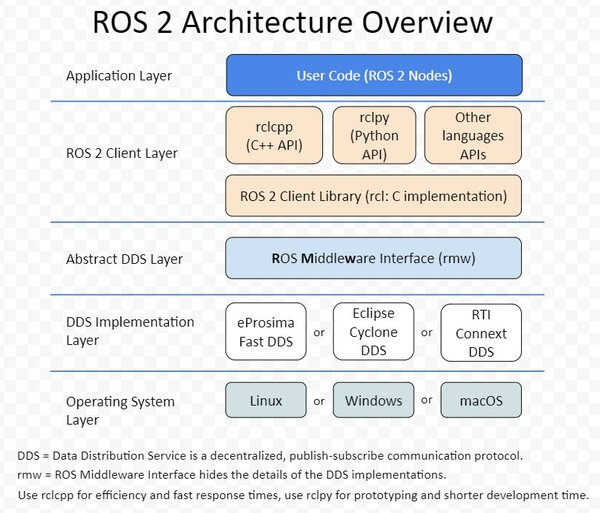
\includegraphics[width=\textwidth]{pictures/ros2_architecture.jpg}



    
    \newpage
    
    \part{Computational Graph Level}


    \section{ROS Master}
        The ROS Master provides name registration and lookup to the rest of the Computation Graph.
        It acts as a nameservice, storing topics and services registration information for nodes. Nodes communicate with the Master to report 
        their registration information.
        As these nodes communicate with the Master, they can receive information about other registered nodes and make connections as appropriate.
        Nodes connect to other nodes directly; the Master only provides lookup information.
        Nodes communication is established over the TCPROS protocol, which uses standard TCP/IP sockets.
        There is always only one master in the network, nodes must know network address of which.


    \section{Nodes}
        Nodes are basic processes that perform computation, written through ROS client library (roscpp, rospy). Each node has its own name 
        (graph resource name) that identify it and a node type (package resource name).
        They are combined into a graph and communicate with each other using:
        \begin{itemize}
            \item topics
            \item services
            \item actions
        \end{itemize}
        Furthermore, they have variables which can be managed using:
        \begin{itemize}
            \item parameter server
            \item dynamic reconfigures
        \end{itemize}    


        \subsection{Python node}
        
            \begin{enumerate}
                \item Package structure
\begin{minted}[bgcolor=LightGray, fontsize=\footnotesize, baselinestretch=1.2]{shell}
/pkg_name
    /nodes
        node.py
    CMakeLists.txt
    package.xml
\end{minted}
            \item Make the node executable
\begin{minted}[bgcolor=LightGray, fontsize=\footnotesize, baselinestretch=1.2]{shell}
chmod +x node.py
\end{minted}

            \end{enumerate}


        \subsection{C++ node}
            \begin{enumerate}
                \item Package structure
\begin{minted}[bgcolor=LightGray, fontsize=\footnotesize, baselinestretch=1.2]{shell}
/pkg_name
    /src
        node.cpp
    /include
        node.h
    CMakeLists.txt
    package.xml
\end{minted}
            \item Make the node executable
\begin{minted}[bgcolor=LightGray, fontsize=\footnotesize, baselinestretch=1.2]{shell}
include_directories(
  include 
  ${catkin_INCLUDE_DIRS}
)
add_excutable(node src/node.cpp)
\end{minted}

            \end{enumerate}





    \section{Communication}


        \begin{tabular}[c]{ |p{2.5cm}||c|p{4cm}|p{3cm}|p{2cm}| }
            \hline
            Messages & Structure  & Application & Example & Tools \\
            \hline
            \hline
            Topics & .msg & one-way continuous data stream & sensors data & rostopic \\
            \hline
            Services & .srv & blocking task for processing a request & trigger, request state, computations & rosservice \\
            \hline
            Actions & .action & non-blocking preemptable goal-oriented tasks & navigation, grasping, motion & actionlib \\
            \hline
            Parameter Server & .param & global constant parameters & names, settings, calibration data, robot setup & rosparam \\
            \hline
            Dynamic reconfigure & .cfg & local, tunable parameters & controller parameters & ?? \\
            \hline
        \end{tabular}


        \subsection{Topics}
            Topics are named buses for unidirectional, streaming communication between nodes, in which there are:
            \begin{itemize}
                \item Publisher – nodes that send data
                \item Subscriber – nodes interested in data
            \end{itemize}
            The master initializes the topic communication and tracks all the information.
            Topics’ default protocol is TCPROS (TCP/IP-based). Another protocol is UDPROS (UDP-based) only for roscpp, that is a low-latency, lossy transport, so is best suited for tasks like teleoperation.
            \\
            Rules:
            \begin{itemize}
                \item Any node can publish a message to any topic
                \item Any node can subscribe to any topic 
                \item Any node can both publish and subscribe to any topics at the same time
                \item Multiple nodes can publish and subscribe to the same topic
            \end{itemize}



        \subsection{Services}
            Services are a pair of messages exchanged between nodes:
            \begin{itemize}
                \item Client (Response) – node providing a service
                \item Server (Request) – node requesting a service which gives back the response
            \end{itemize}
            Rules:
            \begin{itemize}
                \item Any node can implement services (server)
                \item Any node can call services (client)
                \item Servers call are synchronous/blocking
            \end{itemize}



        \subsection{Actions}
            Actions, like services, are messages exchanged between two nodes, providing additional features:
            \begin{itemize}
                \item ActionClient – node providing a task and the possibility to cancel that task
                \item ActionServer – node receiving a task which give back the status, the result and the feedback
            \end{itemize}
            The used protocol is the “ROS Action Protocol” which is built on top of ROS messages (High-level).
            
            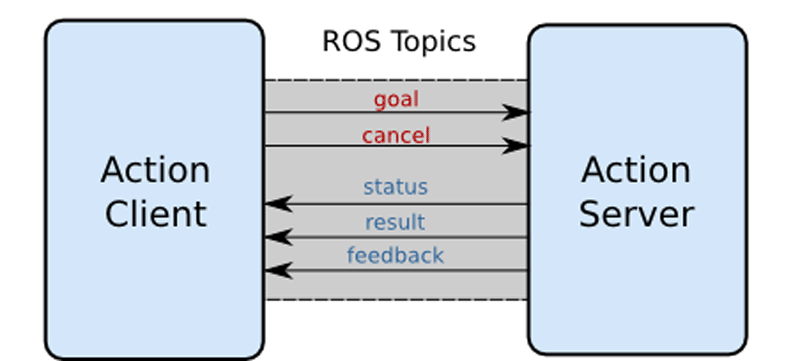
\includegraphics[width=16cm]{pictures/comm_actions.png}
            
            Rules:
            \begin{itemize}
                \item Goal - can be messages, services or parameters data structures used to send goals
                \item Cancel – used to send cancel requests
                \item Status – used to notify clients on the current state of every goal in the system
                \item Feedback - provides information about the incremental progress of a goal
                \item Result - send upon completion of the goal
            \end{itemize}



        \subsection{Parameter Server}
            A parameter server is a shared, multi-variate dictionary implemented using XMLRPC. Nodes can use this server to store and retrieve parameters runtime, for static, non-binary data.
            Supported types:
            \begin{itemize}
                \item strings
                \item 32-bit integers
                \item doubles
                \item float
                \item booleans
                \item lists of elements
                \item dictionary
                \item base64-encoded binary data
                \item iso8601 dates
            \end{itemize}

        
        
        \subsection{Dynamic reconfigure}
            The dynamic reconfigure is a package providing a means to update parameters at runtime without having to restart the node.

            CMakeLists.txt
\begin{minted}[bgcolor=LightGray, fontsize=\footnotesize, baselinestretch=1.2]{xml}
generate_dynamic_reconfigure_options(
    cfg/dynamic.cfg
)
\end{minted}

%             ## CMakeLists.txt
% ```
% # Dynamic reconfigure
% generate_dynamic_reconfigure_options(
%   cfg/dynamic.cfg
% )
% ```
        






    \section{Bags}
        It’s a format for saving, storing and playback ROS message data in .bag files.
        Bag files can be played back in ROS to the same topic they were recorded from, or even remapped to new topics.

    

    \section{Launch files}




        


    
    \newpage
    
    \part{Filesystem}


    %%%%%%%%%%%%%%%%%%%%%%%%%%%%%%%%%%%%%%%%%%%%%%%%%%%%%%%%%%
    %%%%%%%%%%%%%%%%%%%%%%%% Package %%%%%%%%%%%%%%%%%%%%%%%%%
    %%%%%%%%%%%%%%%%%%%%%%%%%%%%%%%%%%%%%%%%%%%%%%%%%%%%%%%%%%
    
    \section{Package}
    
        The package is the smallest unit that is possible to build in ROS and the main unit for organizing software, which can contain:
        \begin{itemize}
            \item ROS runtime processes (nodes)
            \begin{itemize}
                \item scripts: contains executables python scripts
                \item src: contains C++ cource code
                \item include: contains headers and libraries needed
                \item launch: contains launch files
            \end{itemize}    
            \item ROS-dependent libraries (dependencies)
            \begin{itemize}
                \item msg: custom messages structure definition
                \item src: custom services structure definition
                \item action: custom actions structure definition
                \item config: configuration files
            \end{itemize}    
            \item Configuration files
            \begin{itemize}
                \item package.xml: manifest file
                \item CMakeLists.txt: CMake build file
            \end{itemize}
            \item Anything else that is usefully organized together
        \end{itemize}    

\begin{minted}[bgcolor=LightGray, fontsize=\footnotesize, baselinestretch=1.2]{shell}
catkin_ws
  /src
    /pkg_name
      /config
        file.config
      /include
        /pkg_name
          header.h
      /scripts
        node.py
      /src
        node.cpp
      /launch
        node.launch
      /msg
        message.msg
      /srv
        message.srv
      /param
        message.param
      /action
        message.action
      package.xml
      CMakeLists.txt
\end{minted}




    
        \subsection{package.xml}
            The package manifest provides metadata about a package, including its name, version, description, license information, dependencies, and other meta information like exported packages.
    
\begin{minted}[bgcolor=LightGray, fontsize=\footnotesize, baselinestretch=1.2]{xml}
<package format="2">

  <name>pkg_name</name>
  <version>1.2.4</version>
  <description>pkg_description</description>
  <maintainer email="maintainer_email">maintainer_name</maintainer>
  <license>[sw license]</license>
  <url>http://ros.org/wiki/pkg_name</url>
  <author>author_name</author>

  <buildtool_depend>catkin</buildtool_depend>
  <depend>roscpp</depend>
  <depend>rospy</depend>

  <depend>...</depend>

</package>
\end{minted}
    
    
    
        \subsection{CMakeLists.txt}
            The CmakeLists file describes the build instructions for the Cmake.

\begin{minted}[bgcolor=LightGray, fontsize=\footnotesize, baselinestretch=1.2]{xml}
########## Informations ##########
cmake_minimum_required()
project(pkg_name)

# Compiler
set(CMAKE_BUILD_TYPE "Release")
include(CheckCXXCompilerFlag)
CHECK_CXX_COMPILER_FLAG("-std=c++11" COMPILER_SUPPORTS_CXX11)
CHECK_CXX_COMPILER_FLAG("-std=c++14" COMPILER_SUPPORTS_CXX14)

if(COMPILER_SUPPORTS_CXX14)
    set(CMAKE_CXX_FLAGS "-std=c++14")
elseif(COMPILER_SUPPORTS_CXX11)
    set(CMAKE_CXX_FLAGS "-std=c++11")
else()
    message(FATAL_ERROR "No C++11 support")
endif()

set(CMAKE_CXX_FLAGS_RELEASE "-O3 -Wall -g")


########## Dependencies ##########
find_package(catkin REQUIRED COMPONENTS 
  rospy
  roscpp
  ...
)


########## Catkin specific configuration ##########
catkin_package(
  DEPENDS rospy roscpp ...
  CATKIN_DEPENDS rospy roscpp ...
)

include_directories(
  include 
  ${catkin_INCLUDE_DIRS}
)

\end{minted}





    %%%%%%%%%%%%%%%%%%%%%%%%%%%%%%%%%%%%%%%%%%%%%%%%%%%%%%%%%%
    %%%%%%%%%%%%%%%%%%%%% Data Structure %%%%%%%%%%%%%%%%%%%%%
    %%%%%%%%%%%%%%%%%%%%%%%%%%%%%%%%%%%%%%%%%%%%%%%%%%%%%%%%%%

    \section{Data Structure}
    
        The message data structure is the specific format used to compose messages:
        \begin{itemize}
            \item .msg – topic data structure
            \item .srv – service data structure
            \item .action – action data structure
        \end{itemize}
        
        
        \subsection{Creating message package}
        
            It is always suggested to create a separate package containing all the custom messages created:
\begin{minted}[bgcolor=LightGray, fontsize=\footnotesize, baselinestretch=1.2]{xml}
catkin create pkg msg_dep -c rospy roscpp message_generation actionlib actionlib_msgs ...
\end{minted}
            with the following architecture:
\begin{minted}[bgcolor=LightGray, fontsize=\footnotesize, baselinestretch=1.2]{shell}
catkin_ws
  /src
    /pkg_name
      /msg
        message.msg
      /srv
        message.srv
      /param
        message.param
      /action
        message.action
      package.xml
      CMakeLists.txt
\end{minted}
        
        
        \subsection{msgs data structure}
\begin{minted}[bgcolor=LightGray, fontsize=\footnotesize, baselinestretch=1.2]{python}
# defining topic message
message_type message_name
\end{minted}
        
        \subsection{srv data structure}
\begin{minted}[bgcolor=LightGray, fontsize=\footnotesize, baselinestretch=1.2]{python}
# defining request message
request_type request_name
---
# defining response message
response_type response_name
\end{minted}

        \subsection{action data structure}
\begin{minted}[bgcolor=LightGray, fontsize=\footnotesize, baselinestretch=1.2]{python}
# defining topic message
# goal definition
goal_type goal_name
---
# result definition
result_type result_name
---
# feedback
feedback_type feedback_name
\end{minted}
        

        \subsection{CMakeLists.txt}
\begin{minted}[bgcolor=LightGray, fontsize=\footnotesize, baselinestretch=1.2]{shell}
find_package(catkin REQUIRED COMPONENTS
  rospy
  roscpp
  message_generation
  actionlib_msgs
)

# Messages data structure
add_message_files(
  DIRECTORY msg
  FILES message.msg
)

# Services data structure
add_service_files(
  DIRECTORY srv
  FILES message.srv
)

# Actions data structure
add_action_files(
  DIRECTORY action 
  FILES massage.action
)

generate_messages(
  DEPENDENCIES ...
  actionlib_msgs
)

catkin_package(
  CATKIN_DEPENDS rospy roscpp message_runtime actionlib_msgs
)
\end{minted}


        \subsection{package.xml}
\begin{minted}[bgcolor=LightGray, fontsize=\footnotesize, baselinestretch=1.2]{xml}
<build_depend>message_generation</build_depend>
<build_export_depend>message_runtime</build_export_depend>
<exec_depend>message_runtime</exec_depend>
<depend>actionlib</depend>
<depend>actionlib_msgs</depend>
\end{minted}





    %%%%%%%%%%%%%%%%%%%%%%%%%%%%%%%%%%%%%%%%%%%%%%%%%%%%%%%%%%
    %%%%%%%%%%%%%%%%%%%%%% Dependencies %%%%%%%%%%%%%%%%%%%%%%
    %%%%%%%%%%%%%%%%%%%%%%%%%%%%%%%%%%%%%%%%%%%%%%%%%%%%%%%%%%

    \section{Dependencies}
        
        Python modules and C++ libraries are dependencies that can be imported in any other package in the workspace.
        
        
        \subsection{Python modules}
        
        
        
        \subsection{C++ libraries}
        
        
        
        
        
        
        

    
    \newpage

    
    \begin{thebibliography}{9}
    
        \bibitem{ROS official} 
            http://wiki.ros.org/ROS/Introduction
        
        % \bibitem{lable_title} 
        % Aithors. 
        % \textit{The \LaTeX\ Companion}. 
        % Addison-Wesley, Reading, Massachusetts, YEAR.
        
    \end{thebibliography}


\end{document}